\chapter{Introduction}
\label{ch:introduction}

\section{Motivation}
\subsection{What got me interested}
When deciding what to do for my dissertation, I wanted to work on something that affects me on a daily basis.
Most days I spend some time on social media so I asked myself the question, ``What can I do with social media?'' The answer hit me
when looking at my instagram for you page (\cref{fig:motivation-example}). 
\begin{figure}[hbtp]
    \centering
    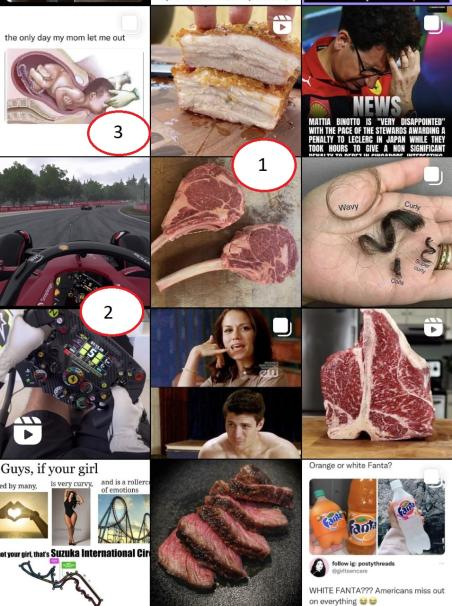
\includegraphics[width=0.6\textwidth]{../images/tweet-example.png}
    \caption{Example tweet}
    \label{fig:motivation-example}
\end{figure}

The content being displayed is all very similar; there is no diversity in the content. This made me ask 3 questions:
\begin{itemize}
    \item What is causing the non-diversity in the content?
    \item Is there any information I can establish about myself from the content?
    \item Is there a way I can force the platform to show me different content?
\captionof{listcap}{Main questions for the project}
\label{list:main-questions}
\end{itemize}

\newpage
\subsection{Where the problem lies}
Answering the first question (Questions \ref{list:main-questions}) was rather simple after some research.
Social media wites use recommender systems to
show users content they are likely to be ``interested'' in \cite{twitter-rec}. Recently Twitter made their recommender system public.
\begin{figure}[hbtp]
    \centering
    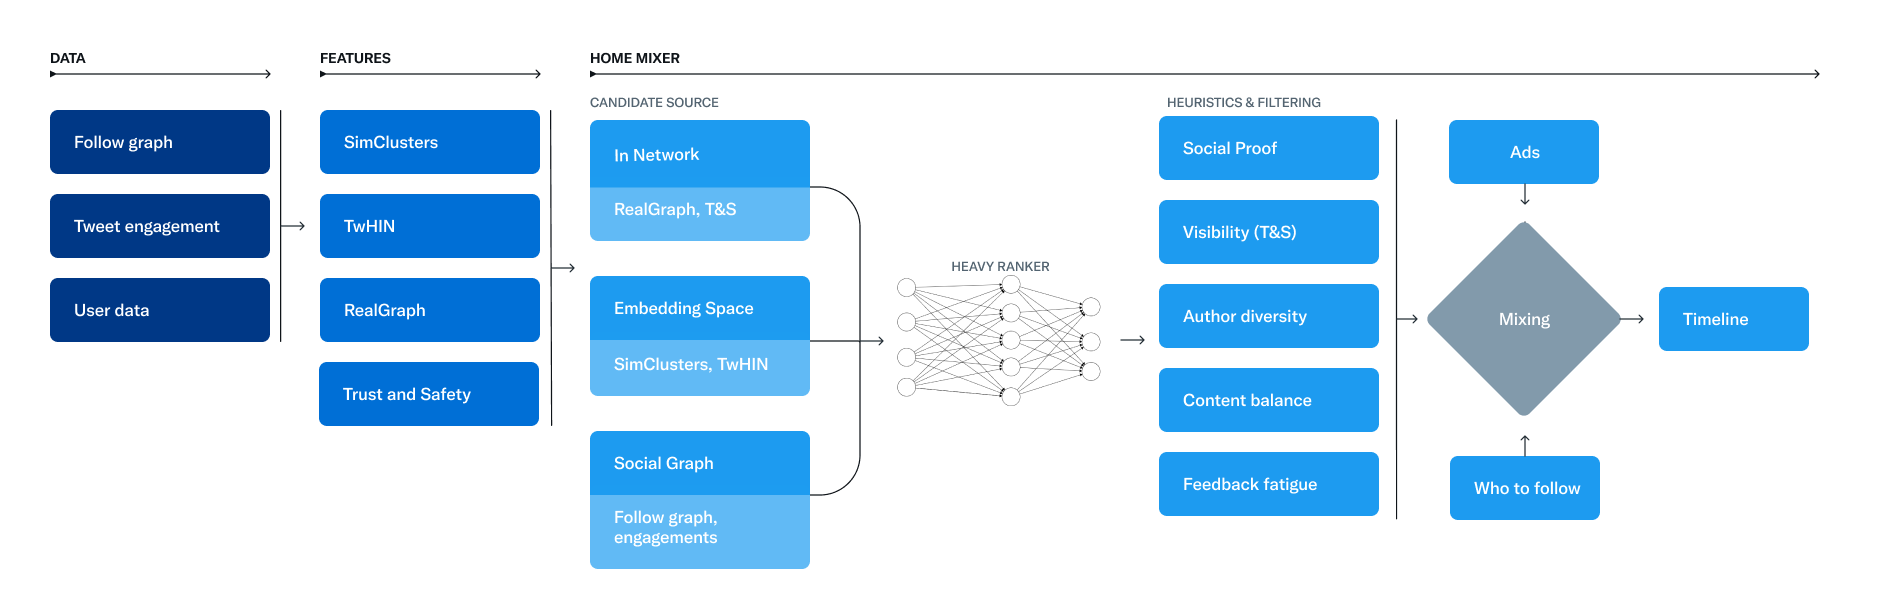
\includegraphics[width=0.8\textwidth]{../images/twitter-recommender.png}
    \caption{Twitter's recommender system}
    \label{fig:twitter-recommender}
\end{figure}

\cref{fig:twitter-recommender} briefly shows how Twitter's recommender system works. The main system is split into three parts;
the first part is `Candidate Sourcing' which selects around 1500 tweets (50\% `in-network' and 50\% `out-of-network'). Secondly,
these posts are ranked using a large neural network. Finally, some heuristics and filters are applied to the ranking.\\
There is already areas here that could cause users to constantly see similar content. This is due to the fact candidate sourcing
is 50\% `in-network'; users are likely to see content created by people they follow. Although this seems mild (due to the other
50\% being `out-of-network') this doesn't necessarily balance out someones feed as the method used to identify candidate
`out-of-network' tweets relies on answering the question ``Who likes similar Tweets to me, and what else have they recently liked?'' \cite{twitter-rec}.
Diving deeper into the heuristics and filters, it is possible to identify another area which would cause users to see similar content
- `Feedback-based Fatigue'. This is where users are not shown posts similar to posts they have negatively interacted with prior.\\
If a user views a certain type of post they are likely to view similar posts in the future \cite{twitter-rec}. With this in mind, it should be possible
to identify a users interests through their social media posts. As a regular user of social media platforms, I have noticed that
the content I see on my feed is always very similar (although may change over larger periods of time). Noticing this, I decided to
play around with how I can force the social media platform to show me differing content. I noticed that (on Instagram) if I simply
chose specific posts to look at on my `for you' page, these posts would be shown to me more often. This shows promise that it is
possible to answer the 3rd question (Questions \ref{list:main-questions}). This experimentation was a large motivating factor
for the original aims of this project set out in my specification (\cref{app:spec}) - to analyse how differing
`strategies' (ways in which someone uses social media) for using social media affect the content shown to the user. However, due to Terms of Service restrictions, this was not
possible. Instead, this project will focus on identifying a users interests through their social media posts. This was an easy transition
as the original project aims required the same prerequisites as this project; both projects need to be able to classify social media posts
into topics. Another benefit of this project is that given permission from social media platforms in the future, it will be possible to
extend this project to analyse `strategies' as set out in the original project aims.\\

\subsection{Why is this a problem?}
Because recommender systems tend to show users content they have (positively) interacted with in the past echo chambers can be created.
Echo chambers are where the ideas and beliefs of a group of people are reinforced through confirmation bias \cite{echo-chambers}.
When a user is scrolling through their social media feed they are likely to pick out posts that they agree with and like/share them \cite{collatt}\cite{misinf}.
This interaction with the post will cause the recommender system to show more of this type of content to the user.
Another, although similar, problem is the spread of misinformation. This is where content that is false is spread to a large number of people \cite{misinf}\cite{misinfspread}.
These people then like/share the content which causes more of the post to be shown to more people. Which can very quickly
spread false information to a large number of people.\\
If it is possible for users to identify how their social media content leans (e.g. political leaning) it allows them to identify
whether they are in an echo chamber and then take steps to resolve this issue.

\section{Problem Statement}
The main crux of this project is attempting to answer the 2nd question (Questions \ref{list:main-questions}). Using the idea
that recommender systems will show users content that they believe the user will be interested in \cite{twitter-rec}, it should be possible to
identify a users interests through their social media feed. This project works on classifying social media posts. This will
allow us to identify interests through comparing similarities between posts shown to the user. This will be followed by quantifying
a set of posts to compare the similarity between a users posts and posts from the entire social media site.
Finally, this project aims to create a user interface that allows users to discover what their social media feed says about their
interests and how they compare to the rest of the social media site. The user interface will also allow users to discover posts
that are dissimilar to the posts they are shown.

\section{Topics}
This project will use the notion of topics to identify what the posts are about.
\begin{figure}[hbtp]
    \centering
    a subject that is discussed, written about, or studied
    \caption{Topic Definition - \cite{cambdict}}
    \label{fig:topic_definition}
\end{figure}

This definition of a topic is a good starting point for this project. This definition is a bit too specific. If this definition were 
to be used there would be no meaningful output from this project - due to the fact you could classify each post into its own unique
topic. To overcome this, we will use a more general definition of a topic. Essentially, a topic comprises of a set of words that
are related to each other and reflect a common theme/subject. For example, the topic of `food' would contain words like `steak',
`chicken', `pizza' etc.


\section{Related work}
\subsection{Latent Dirichlet Allocation - \cite{latentDirAll}}
Latent Dirichlet Allocation (LDA) is a generative probabilistic model that is used to classify documents into topics \cite{latentDirAll}. LDA aims to find a set of topics that are representative of the documents
in a corpus. It does this by assigning each word in a document to a topic and then assessing the following probabilities:
\begin{itemize}
    \item $p(\text{topic t} \vert \text{document d})$ - The probability of a topic being assigned to a document
    \item $p(\text{word w} \vert \text{topic t})$ - The probability of a word being assigned to a topic
\end{itemize}

LDA then uses Gibbs sampling to assign each word in a document to a topic based on the above probabilities. Below is a
simplified version of the LDA algorithm to give some intuition on how it works
\begin{equation}
    p(\text{word w with topic t}) = p(\text{topic t} \vert \text{document d}) * p(\text{word w} \vert \text{topic t})
\end{equation}

LDA is a very powerful unsupervised learning technique that can be used to classify documents into topics. However,
it has some limitations (due to it being an unsupervised technique) that will be discussed in \cref{sec:topic_modelling}.
\subsection{Pythia - \cite{Pythia}}
\label{sec:pythia}
Pythia is an automated system for short text classification. It makes use of Wikipedia structure and articles to identify
topics of posts.
Essentially, ``Wikipedia contains articles organized in various taxonomies, called categories''. Pythia then goes on to use
this information as their training data as well as handling sparseness in posts on social media.\\

Pythia also demonstrates a method to overcome the lack of context in short texts - This is a large problem in identifying
smaller social media posts like tweets, and will be further worked on in this project. They use a method called ``Post Enrichment'',
which performs i) Named Entity Recognition then ii) Lemmatization and stop word removal. We then use the named entities to query
wikipedia for similar articles that are then appended to the post.\\

Although this method works well in cases where keywords are used, there are cases where no keywords are used, and more context
is needed. Take for example the following tweet:
\begin{figure}[htbp]
    \centering
    
\includegraphics[width=0.6\textwidth]{../images/tweet-example2.png}
    \caption{Example tweet}
    \label{fig:tweet-example}
\end{figure}

The text gives us very little context; What is this tweet about? the best guess could be
is it is a message to other users. If these users had wikipedia articles, we could use them. But in reality this post is about something else.
Lets add some other form of context; add the media the tweet contains.
\newpage
\begin{figure}[hbtp]
    \centering
    
\includegraphics[width=0.6\textwidth]{../images/tweet-media.png}
    \caption{Example tweet - media}
    \label{fig:tweet-media}
\end{figure}
This gives us a lot more context; the tweet is discussing the earthquake that hit Turkey and Syria, if we use this for our query we get more relevant
articles:

\begin{figure}[htbp]
    \centering
    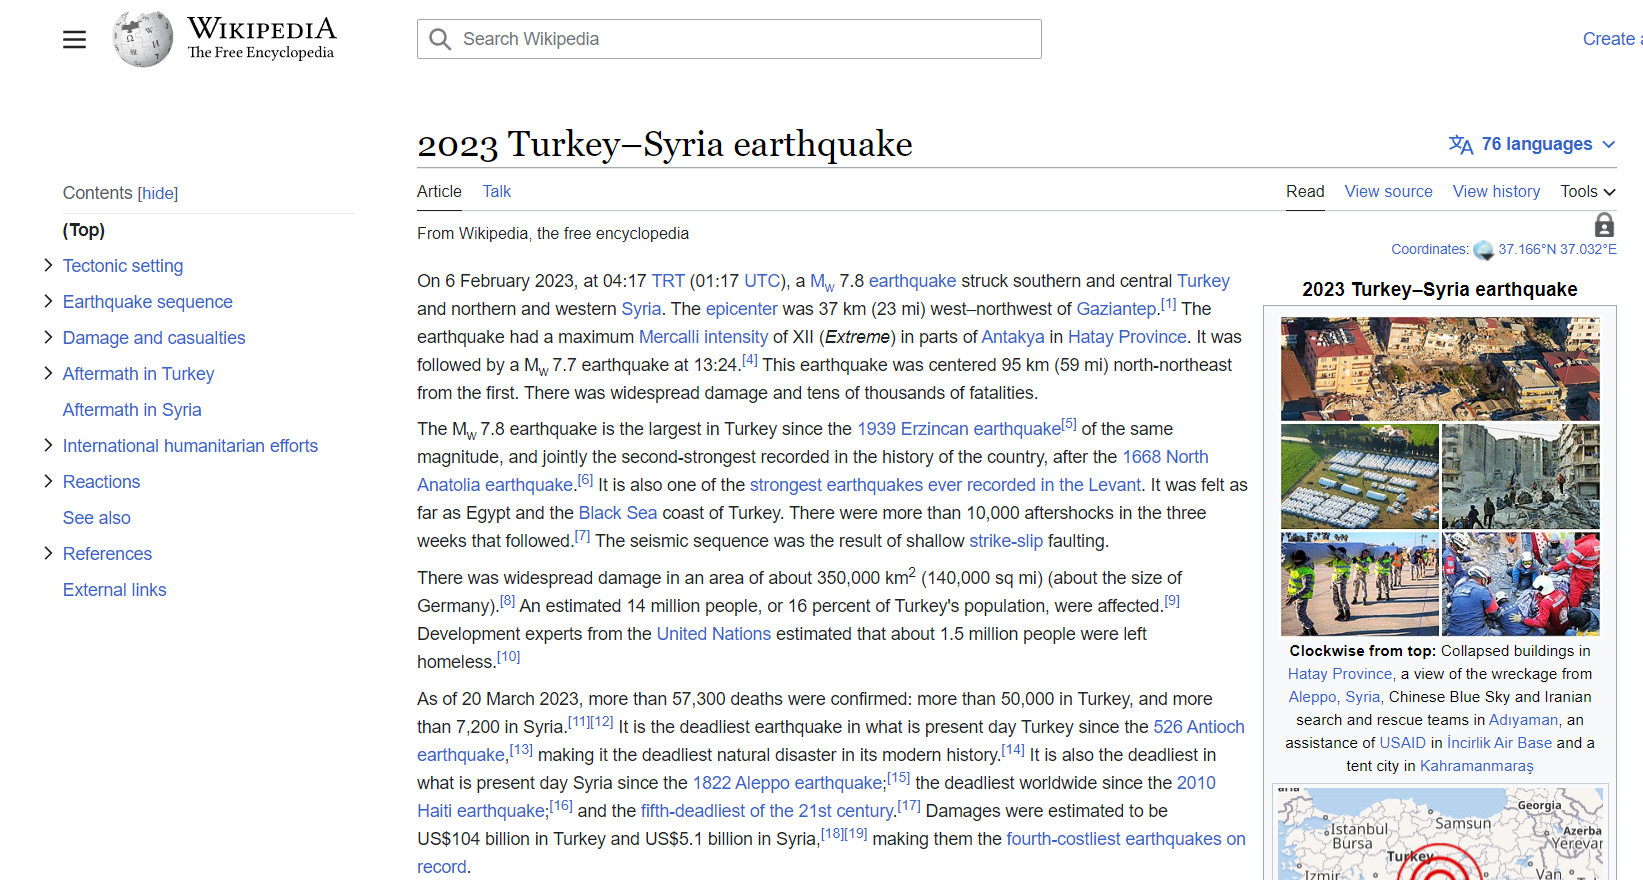
\includegraphics[width=0.6\textwidth]{../images/post-context-example.png}
    \caption{Wikipedia articles relating to the Syria Turkey earthquake}
    \label{fig:blastpremier}
\end{figure}

We now have a lot of relevant information to append to the post. We could use other information for context as well: Tweet author,
images/media in tweets, retweet information, like information, etc.

\subsection{Deep Short Text Classification with Knowledge Powered Attention - \cite{DeepShortText}}
Following on from the work of adding context in \cref{sec:pythia}, this paper proposes a more sophisticated method of adding
conceptual information via Knowledge Bases (KBs). Knowledge Bases are a store of information/rules that an AI/ML model can use
to make decisions \cite{kb}. A knowledge base system isn't programmed to solve a specific problem, but rather it is given a
set of declarative rules that it can use to solve a problem \cite{kb}. They make use of a method called ``Knowledge Powered Attention'' (KPA) to
incorporate KBs into their model. What is Knowledge Powered Attention?\\
\begin{figure}[hbtp]
    \centering
    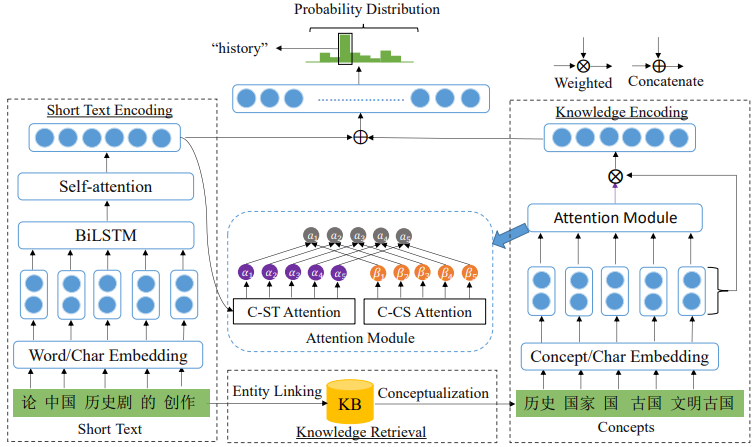
\includegraphics[width=0.6\textwidth]{../images/kpa.png}
    \caption{Knowledge Powered Attention architecture}
    \label{fig:kpa}
\end{figure}

\cref{fig:kpa} show the architecture proposed by the paper. There are several separated modules, but to understand how Knowledge
is used, the focus will be on:
\begin{itemize}
    \item Knowledge Retrieval
    \item Attention Model
\end{itemize}

\subsubsection{Knowledge Retrieval}
The premise of this module is to take a short text $s$ and retrieve a `concept set' $C$. There are two steps to this:
\begin{enumerate}
    \item Entity Linking
    \item Concept Set Retrieval
\end{enumerate}

Entity Linking is used to identify the entities mentioned in the short text \cite{DeepShortText}.\\
Concept Set Retrieval uses the entities found in the previous step and queries a KB to find the concepts related to the entities.

\subsubsection{Attention Model}
The attention model comprises of 2 separate attention mechanisms called: `Concept towards Short Text (C-ST) Attention' and 
`Concept towards Concept Set (C-CS) Attention'.\\
C-ST attention is put in place to attempt to reduce the bad influence from improper concepts in the concept set. It does this
by measuring the semantic similarity between the concepts and the short text. The paper uses `vanilla' attention and does
not elaborate what is meant by this. Nonetheless, the idea of measuring similarity of a set based on information from
another set could perform better using cross-attention mechanisms. Cross-attention could work well due to the fact it uses
the set being compared against to fill the `Key' and `Value' vectors. Then use the set being compared as the `Query' \cite{attention}.
This in-built separation shows how cross-attention could work well in this case.\\
C-CS attention is put in place to measure how important each concept is relative to the other concepts. It uses basic
self-attention to do this.\\
The two attention mechanisms are then combined to form the final attention vector used for the knowledge embeddings using the equation
in \cref{eq:attention_combination}.
\begin{equation}
    a_i = softmax(\gamma\alpha_i + (1-\gamma)\beta_i)
    \caption{Combining C-ST and C-CS attention}
    \label{eq:attention_combination}
\end{equation}

where $\gamma$ is a hyperparameter to control the importance of each attention mechanism.

\subsection{Topic tracking of student-generated posts - \cite{TopicTracking}}
This paper proposes a solution for determining valuable information/topics discussed in student forums on online courses.
It uses a model called ``Time Information-Emotion Behaviour Model'' or otherwise called ``TI-EBTM'' to detect key topics discussions
, keeping in mind the progress of time throughout the forum.\\
The concept that time is important in determining the topic of a post is a good one. It could be possible
to incorporate a time-sensitive model into the project to determine the topic of a post. This is not done in this project
but is a good idea for future work.

\subsection{Topic classification of blogs - \cite{husby2012topic}}
This paper uses Distant Supervision - 'an extension of the paradigm used by \cite{snow} for exploiting WordNet to extract hypernym (is-a) relations between entities'
- to get training data via Wikipedia articles. Then trains their own designed model on this data to be able to classify topics via a
multi-class recognition model (69\% accuracy) and via a binary classification model (90\% accuracy).

\section{Objectives}
To achieve the problem statement, the following objectives must be met:
\begin{itemize}
    \item Generate a list of topics for classification
    \item Implement methods for identifying the topics in social media posts
    \item Compare and contrast the results of the different methods
    \item Create a user interface
    \begin {itemize}
        \item Allow users to compare their interests to the rest of the social media site
        \item Allow users to discover posts that are dissimilar to the posts they are shown
    \end{itemize}
\end{itemize}
The largest problem with this project is the second objective of finding and creating methods for identifying topics.